\documentclass[conference]{IEEEtran}
\IEEEoverridecommandlockouts
\usepackage{cite}
\usepackage{amsmath,amssymb,amsfonts}
\usepackage{algorithm}
\usepackage{algorithmic}
\usepackage{graphicx}
\usepackage{textcomp}
\usepackage{xcolor}
\usepackage{booktabs}
\usepackage{array}
\usepackage{url}
\usepackage[hidelinks]{hyperref}
\usepackage{caption}
\captionsetup{font=footnotesize,labelsep=period,justification=raggedright,singlelinecheck=true}
\captionsetup[table]{textfont=normalfont,labelfont=bf,justification=raggedright,singlelinecheck=true}
\renewcommand{\tablename}{Table}
\renewcommand{\figurename}{Fig.}
\graphicspath{{figs/}}

% arabic (not roman) table and figure numbers
\renewcommand{\thetable}{\arabic{table}}
\renewcommand{\thefigure}{\arabic{figure}}

\newcolumntype{C}[1]{>{\centering\arraybackslash}p{#1}}
\newcommand{\best}[1]{\textbf{#1}}

\begin{document}

\title{Auditing Accuracy, Explanation Fidelity, and Robustness for Trustworthy UAV Power Prediction}

% ===== DOUBLE-BLIND SUBMISSION: authors anonymised for ICTAI review. =====
% For the camera-ready (after acceptance), replace the anonymous block below
% with the real author block (names, affiliations, emails, ORCIDs).
\author{%
\IEEEauthorblockN{Anonymous Author(s)}
\IEEEauthorblockA{Affiliation(s) withheld for double-blind review}}


\maketitle

\begin{abstract}
Practitioners routinely pick a machine-learning estimator of unmanned aerial vehicle (UAV) power draw by whichever regressor reports the smallest prediction error. That habit is a shaky foundation for a decision that governs range planning and the in-flight call to press on or abort. A model can edge ahead on accuracy yet attribute its predictions to the wrong drivers, and it can fall apart under the sensor noise that real telemetry always carries; an error table shows neither problem. We therefore recast model selection for safety-relevant UAV power prediction as an audit along three axes at once: predictive accuracy, explanation fidelity, and robustness. Four findings on a public flight-telemetry data set of 188 flights support the case. First, we introduce Robust Anchored Stacking, a non-negative blend of two gradient boosters and a linear anchor with base learners trained on noise-augmented telemetry. It posts the lowest error on every leakage-free split, is the most robust among the accurate models, and ties for the most faithful black-box attribution, which lets it Pareto-dominate every baseline across all three axes simultaneously. Second, an audit of three standard tree explainers along fidelity, deletion faithfulness, and stability identifies the one best matched to this tabular, tree-based setting. Third, we surface a failure that accuracy hides: a popular booster whose error almost doubles under modest noise. Finally, we combine the three axes into a Unified Trust Score and a Pareto analysis, turning a flat leaderboard into a transparent, mission-aware deployment choice that we operationalise through a serving architecture and an operator-facing tool. Every number we report comes from executed code on the real data.
\end{abstract}

\begin{IEEEkeywords}
UAV power prediction, explainable AI, explanation fidelity, robustness, stacking ensembles, multi-criteria decision analysis, trustworthy machine learning.
\end{IEEEkeywords}

\section{Introduction}
Knowing the instantaneous electrical power a UAV draws is a precondition for flying it safely: range prediction, payload planning, and the mid-mission choice to continue or abort all rest on it~\cite{stolaroff2018energy,thibbotuwawa2020energy}. Recent work tends to follow a fixed recipe, namely benchmark a few regressors, keep the one with the smallest mean absolute error (MAE), and move on. Our view is that accuracy alone makes a thin case for a safety-relevant deployment, and that two other properties belong on the same footing. One is explanation fidelity. When an operator or a certification body relies on an attribution claiming that payload dominates power draw, that attribution has to track the model itself, not the idiosyncrasies of whichever explainer produced it~\cite{jacovi2020towards,rudin2019stop}. The other is robustness. A model that is accurate on clean telemetry but comes apart the moment an anemometer or accelerometer drifts is a hazard rather than an asset~\cite{hendrycks2019benchmarking}.

An earlier study on the same data set compared several models, picked the most accurate booster, and noted in passing that a neural baseline broke down under noise. We take that as a useful point of departure, but three gaps in it motivate our work. Its choice hinged on one criterion. It measured explanation fidelity for a single explainer, which leaves unclear whether the reported fidelity belonged to the model or to the explainer. And it stopped short of converting the accuracy, fidelity, and robustness signals into a selection procedure that an engineer could actually run and reproduce.

Those gaps translate into the three questions our study is built around. Can a carefully constructed learner beat strong single boosters such as CatBoost on accuracy without giving up explanation fidelity or robustness? Among the explanation methods in common use, which is the most faithful in this tabular, tree-based regime? And do the accuracy, fidelity, and robustness rankings line up at all, so that when they pull in different directions we know how a deployment model ought to be chosen?

Taken together, the answers to these questions form the paper's contributions. Robust Anchored Stacking is the most accurate model on every leakage-free split we ran, while it stays the most robust of the accurate models and ties for the most faithful black-box attribution, so that it Pareto-dominates every black-box baseline across all three axes at once. Building on that ensemble, we audit three standard tree explainers against a physics-grounded reference, a reference-free deletion criterion, and stability under noise, and single out the one best suited to this setting. Beyond model choice, we expose a robustness failure that accuracy masks, since an otherwise competitive booster gives up 44\% of its accuracy under modest noise, which is precisely why robustness warrants its own axis. To close the loop, we fold the three axes into a Unified Trust Score and a Pareto analysis that return a short list of deployment-ready models, and we back the result with a serving architecture and an operator-facing tool. The pipeline from raw input to a risk-stratified recommendation is laid out in Fig.~\ref{fig:arch}.

\begin{figure*}[t]
\centering
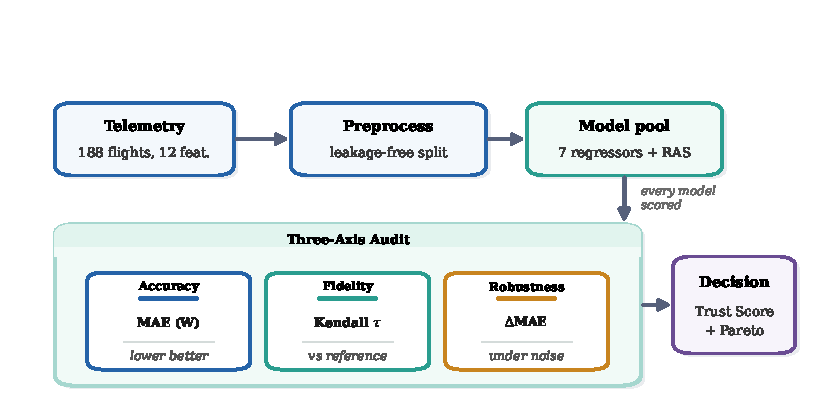
\includegraphics[width=0.84\textwidth]{fig_architecture.pdf}
\caption{The proposed audit at a glance. Flight telemetry is split without leakage and standardised, a pool of seven regressors plus the proposed ensemble is built, and each model is scored on three independent axes, namely accuracy, explanation fidelity, and robustness. A multi-criteria stage then normalises the scores, finds the non-dominated set, and returns a risk-stratified recommendation with a consensus rationale.}
\label{fig:arch}
\end{figure*}

\section{Related Work}
Energy estimation for multirotors has been pursued both from physics and from data, and the recent balance has tipped toward learned models fitted to telemetry, since they pick up aerodynamic and payload effects that analytic battery and aerodynamic models capture only roughly~\cite{rodrigues2021drone,abeywickrama2018comprehensive,zeng2019energy}. Our question sits to one side of that accuracy race: we ask what else a model must satisfy before anyone trusts it in the loop. For the estimator itself, gradient-boosted trees are still the front-runner on tabular regression~\cite{grinsztajn2022why,shwartzziv2022tabular}, and stacked generalisation blends complementary learners through a meta-model~\cite{wolpert1992stacked,dietterich2000ensemble}. Our reason for stacking is not only accuracy, since its explicit weights also give a principled route to combining the bases' attributions and to anchoring the ensemble with a robust linear term. Because those weights are non-negative and sum to one, each base's contribution to the blend stays directly readable, and it is exactly this readability that later lets us attribute the ensemble as faithfully as its individual bases, so the meta-model here is chosen for transparency as much as for capacity.

A second thread concerns whether explanations are faithful at all, and it is now large enough to have its own surveys~\cite{guidotti2018survey,arrieta2020explainable}. Additive feature attributions, above all SHAP and its exact tree variant~\cite{lundberg2017unified,lundberg2018consistent}, sit alongside gradient and surrogate methods in everyday use~\cite{ribeiro2016why}. Their faithfulness, though, is neither guaranteed nor independent of the estimator and the method that produced them~\cite{jacovi2020towards}: post-hoc explainers have flunked basic sanity checks~\cite{adebayo2018sanity} and have been steered by adversaries~\cite{slack2020fooling}, which is why some have argued that explanations should face the same scrutiny as the models~\cite{doshivelez2017towards}. Deletion-style metrics track how fast predictions decay once the top-ranked features are removed~\cite{hooker2019benchmark}; this reference-free view is the one we use to referee competing explainers, and the hazard of trusting any single explainer is by now well established~\cite{krishna2022disagreement}. Where one response has been to build models interpretable from the outset~\cite{caruana2015intelligible}, we instead keep strong black boxes but put their explanations through an audit, adding a robustness lens for corrupted inputs~\cite{hendrycks2019benchmarking} and multi-criteria decision analysis to trade off competing desiderata~\cite{hwang1981multiple} within a single selection procedure.

\section{Methodology}

\subsection{Data and Features}
The data come from a public quadrotor flight-telemetry set covering 188 flights in cruise, takeoff, and landing~\cite{rodrigues2021drone}. We regress instantaneous electrical power, taken as battery voltage times current. Dropping degenerate flights and rows with missing kinematics leaves 177{,}464 samples. We engineer nine predictors, namely payload, commanded speed, altitude setpoint, wind speed, velocity magnitude, acceleration magnitude, angular-rate magnitude, pitch, and headwind, and add a one-hot encoding of the flight regime, for twelve features in all. To keep telemetry from one flight leaking across the split, we partition by flight identifier in an 80/20 grouped fashion, so no flight lands in both train and test, and we standardise using statistics computed on the training partition only. Every model is built with scikit-learn and the matching gradient-boosting libraries~\cite{pedregosa2011scikit}.

\subsection{Models and the Proposed Ensemble}
Across the study we evaluate seven regressors, and we deliberately leave out the baseline's multilayer perceptron, since a stronger and more instructive cautionary case takes its place later (Section~\ref{sec:robust}). Table~\ref{tab:models} lists the pool and its configurations, namely a regularised linear model (Ridge), a random forest, gradient boosting, and three modern gradient boosters, CatBoost~\cite{prokhorenkova2018catboost}, XGBoost~\cite{chen2016xgboost}, and LightGBM~\cite{ke2017lightgbm}.

Robust Anchored Stacking parts ways with a plain booster stack in three deliberate choices. It first removes XGBoost from the bases, since our robustness audit flags it as the single most fragile learner in the pool. It then keeps the two remaining boosters, CatBoost and LightGBM, and pairs them with a Ridge anchor so that a smooth linear term always sits in the blend. The third choice matters most for robustness: each base learner sees noise-augmented telemetry, because we concatenate the training set with one Gaussian-perturbed copy of itself, and this teaches the bases to shrug off the small sensor drift the robustness probe applies afterward. We combine the bases with non-negative weights from non-negative least squares on a flight-grouped holdout, which keeps the mixture transparent and easy to read; on the canonical split those weights come out to 0.40 for CatBoost, 0.56 for LightGBM, and 0.04 for the Ridge anchor. The same weights carry over to explaining the ensemble, where the bases' exact TreeSHAP magnitudes and the anchor's coefficients merge into one faithful attribution. Algorithm~\ref{alg:ras} gives the full procedure.

\begin{algorithm}[t]
\caption{Robust Anchored Stacking (training)}
\label{alg:ras}
\small
\begin{algorithmic}[1]
\REQUIRE training features $X$, target $y$, flight groups $g$, noise scale $\varepsilon$
\STATE $\mathrm{aug}(A,b)\!:=\![\,A;A{+}\varepsilon\mathcal{N}(0,I)\,],[\,b;b\,]$ \COMMENT{noise replica}
\STATE split $(X,y)$ by group into fit set $F$ and holdout $H$
\STATE fit CatBoost, LightGBM, Ridge on $\mathrm{aug}(X_F,y_F)$
\STATE $P \leftarrow$ base predictions on $H$
\STATE $w \leftarrow \arg\min_{w\ge 0}\lVert Pw - y_H\rVert_2$; \; $w \leftarrow w/\textstyle\sum_i w_i$ \COMMENT{NNLS}
\STATE refit CatBoost, LightGBM, Ridge on $\mathrm{aug}(X,y)$
\ENSURE bases and weights $w$; predict by $\hat{y}(x)=\sum_i w_i\,\mathrm{base}_i(x)$
\end{algorithmic}
\end{algorithm}

\begin{table}[t]
\centering
\caption{Model pool and configuration. The multilayer perceptron of the baseline is excluded.}
\label{tab:models}
\small
\begin{tabular}{@{}lll@{}}
\toprule
Model & Family & Key configuration \\
\midrule
Ridge & Linear & $\alpha=1.0$ \\
Random Forest & Bagged trees & 300 trees, min leaf 5 \\
Gradient Boosting & Boosted trees & 300 rounds, depth 5 \\
CatBoost & Boosted trees & 500 rounds, depth 6 \\
XGBoost & Boosted trees & 600 rounds, depth 6, hist \\
LightGBM & Boosted trees & 600 rounds, 63 leaves \\
RAS (ours) & Anchored stack & CatBoost, LightGBM, Ridge \\
\bottomrule
\end{tabular}
\end{table}

\subsection{Explanation Fidelity and Method Audit}
Because we want fidelity anchored in physics rather than in another learned model, the absolute, normalised Ridge coefficients serve as a soft ground-truth importance over the twelve features, a choice justified by the near-linear way payload and a handful of kinematic terms govern power. For any attribution we then take its Kendall-$\tau$ rank agreement with this reference~\cite{kendall1938new}, which asks only whether the explanation orders the drivers correctly. The explainer itself is audited on its own terms, and here the three global methods standard in a tabular, tree-based setting are exact TreeSHAP, permutation importance, and impurity gain, whereas gradient- and surrogate-based attributions like Grad-CAM and Anchors target other model families~\cite{selvaraju2017gradcam} and are not a natural fit. Each method is then read through three lenses at once: its agreement with the physics reference; a reference-free deletion criterion, under which features are removed most-relevant-first, each replaced by its training mean, so that the area under the resulting error-increase curve measures how hard the top features actually drive the model~\cite{hooker2019benchmark}; and its stability, the rank agreement between an explanation on clean inputs and on inputs perturbed by 10\% noise~\cite{alvarezmelis2018robustness}. A trustworthy explainer should score well on all three together.

\subsection{Evaluation Protocol}
\label{sec:robust}
Accuracy is reported as MAE, root mean squared error (RMSE), and the coefficient of determination on the held-out flights. A single grouped split can flatter a model by luck, so we redraw the split under five seeds, report the mean and standard deviation of MAE, and compare the proposed model with the best single booster using a paired Wilcoxon signed-rank test over the five splits~\cite{wilcoxon1945individual}. For robustness we add zero-mean Gaussian noise at growing scale to the standardised test features and record the relative MAE degradation at 5\%, 10\%, and 20\% noise, averaged over five noise draws; this stands in for the sensor drift and calibration error a deployed model would meet. To bring the axes back together, we min--max normalise each criterion to $[0,1]$, orienting accuracy and robustness so that larger is better, and define the Unified Trust Score (UTS) as the weighted sum of a model's normalised accuracy, fidelity, and robustness. Three mission profiles follow, performance-critical, balanced, and safety-critical, with weight vectors $(0.60,0.20,0.20)$, $(0.34,0.33,0.33)$, and $(0.20,0.50,0.30)$. We then read off the Pareto-optimal set, the models not dominated on all three axes together, and measure how far the criteria agree with the Spearman rank correlation of their orderings~\cite{spearman1904proof}.

\section{Results}

\subsection{Accuracy}
Turning to the measurements, Table~\ref{tab:acc} reports predictive accuracy, and the proposed ensemble records the lowest error at 40.82~W on the canonical split, edging out CatBoost at 41.01~W and the other boosters, with Ridge well behind at 47.90~W. In absolute terms the lead is slim, yet it holds up, because over five leakage-free splits the ensemble owns the lowest mean MAE ($38.07 \pm 1.54$~W) and beats CatBoost on all five. Against CatBoost the paired Wilcoxon test returns $p=0.0625$, the floor for five paired samples, which signals a clean five-of-five win rather than a borderline one. We read this as a qualified yet genuine yes to the first question, in that a well-built ensemble does improve on the strongest single booster, even if the margin is modest and best not oversold.

\begin{table}[t]
\centering
\caption{Predictive accuracy. Multi-seed columns are mean$\pm$std over five leakage-free splits. Best per column in bold.}
\label{tab:acc}
\small
\begin{tabular}{@{}lcccc@{}}
\toprule
Model & MAE & MAE (5 splits) & RMSE & $R^2$ \\
 & (W) & mean$\pm$std & (W) & \\
\midrule
RAS (ours) & \best{40.82} & \best{38.07$\pm$1.54} & \best{58.54} & \best{0.622} \\
CatBoost & 41.01 & 38.39$\pm$1.48 & 58.67 & 0.620 \\
LightGBM & 41.19 & 38.19$\pm$1.66 & 59.37 & 0.611 \\
XGBoost & 41.27 & 38.21$\pm$1.70 & 59.42 & 0.611 \\
Gradient Boosting & 41.68 & 38.73$\pm$1.65 & 59.88 & 0.605 \\
Random Forest & 42.05 & 39.44$\pm$1.48 & 60.48 & 0.597 \\
Ridge & 47.90 & 44.85$\pm$1.72 & 71.43 & 0.437 \\
\bottomrule
\end{tabular}
\end{table}

\subsection{Robustness}
Robustness, gathered in Fig.~\ref{fig:robust} and the robustness column of Table~\ref{tab:scorecard}, is a more sobering read than accuracy on its own. Ridge stays the steadiest by a wide margin, losing just 2.8\% of its accuracy at 20\% noise, as a smooth linear response should. The boosters, by contrast, split apart: CatBoost degrades gently at 16.4\%, while LightGBM and above all XGBoost do markedly worse. XGBoost is the case worth dwelling on. It is competitive on clean data yet forfeits 44.3\% of its accuracy under noise, with most of the harm done already at 5\%, where its error jumps from 41.3~W to 54.5~W. We call this the most consequential practical result of the audit, because the trap is invisible to anyone who reads the accuracy column alone: the original baseline flagged a neural model as fragile, and here the very same fragility hides inside a far more popular and respected booster. Set against that, the proposed ensemble is the most robust of all the accurate models, rising only 14.2\% at 20\% noise and bettered by Ridge alone, and the ablation in Table~\ref{tab:ablation} shows where the robustness comes from. Noise augmentation does the heavy lifting: strip it out and the same blend slips to 18.5\% with no accuracy penalty, so the extra invariance is essentially free. The Ridge anchor plays a quieter but intentional part; removing it trims a negligible 0.03~W off the error but drops explanation fidelity from 0.636 to 0.606, an accuracy-for-faithfulness swap we are unwilling to make in a safety context. Adding XGBoost back as a fourth base moves none of the three metrics yet drags the brittle learner into the blend at a non-trivial weight, confirming that leaving it out costs nothing and closes off a latent failure mode.

\begin{table}[t]
\centering
\caption{Three-axis trust scorecard for the held-out flights. Arrows mark the preferred direction of each axis; the final column flags membership of the Pareto-optimal (non-dominated) set. Best per column in bold.}
\label{tab:scorecard}
\small
\resizebox{\columnwidth}{!}{%
\begin{tabular}{@{}lcccc@{}}
\toprule
Model & MAE (W) $\downarrow$ & Fidelity $\tau$ $\uparrow$ & $\Delta$MAE @20\% $\downarrow$ & Pareto \\
\midrule
\textbf{RAS (ours)} & \best{40.82} & 0.636 & 14.2\% & \checkmark \\
CatBoost & 41.01 & 0.606 & 16.4\% & \\
LightGBM & 41.19 & 0.606 & 26.7\% & \\
XGBoost & 41.27 & 0.636 & 44.3\% & \\
Gradient Boosting & 41.68 & 0.576 & 17.0\% & \\
Random Forest & 42.05 & 0.515 & 18.9\% & \\
Ridge & 47.90 & \best{0.970} & \best{2.8\%} & \checkmark \\
\bottomrule
\end{tabular}%
}
\end{table}

\begin{table}[t]
\centering
\caption{Ablation of Robust Anchored Stacking on the canonical split, isolating each design choice along the three axes. Removing the noise augmentation leaves accuracy untouched but degrades robustness; removing the Ridge anchor buys a negligible 0.03~W of accuracy at a real cost in explanation fidelity; and adding an XGBoost base changes nothing while reintroducing the brittle learner the design deliberately excludes. The full configuration is the best compromise across all three axes.}
\label{tab:ablation}
\small
\resizebox{\columnwidth}{!}{%
\begin{tabular}{@{}lccc@{}}
\toprule
Variant & MAE (W) $\downarrow$ & $\Delta$MAE @20\% $\downarrow$ & Fidelity $\tau$ $\uparrow$ \\
\midrule
\textbf{RAS (full)} & 40.82 & 14.2\% & 0.636 \\
\quad $-$ noise augmentation & 40.84 & 18.5\% & 0.636 \\
\quad $-$ Ridge anchor & 40.79 & 14.6\% & 0.606 \\
\quad $+$ XGBoost base & 40.83 & 14.2\% & 0.636 \\
\bottomrule
\end{tabular}%
}
\end{table}

\begin{figure}[t]
\centering
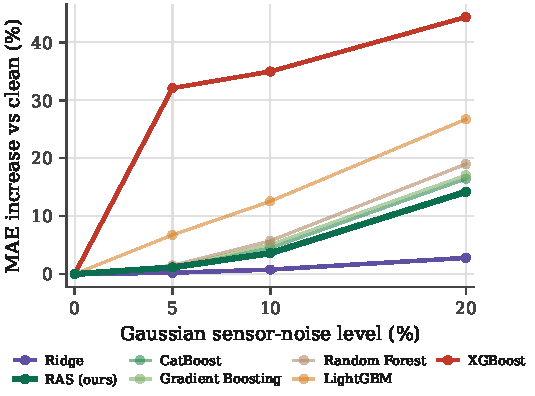
\includegraphics[width=0.99\columnwidth]{fig_robust.pdf}
\caption{Relative MAE increase versus clean data as Gaussian sensor noise grows. XGBoost is brittle, degrading sharply at the lowest noise level, whereas the proposed ensemble stays close to the linear Ridge baseline.}
\label{fig:robust}
\end{figure}

\subsection{Explanation Fidelity}
Accuracy and fidelity turn out to move more or less independently, as the fidelity column of Table~\ref{tab:scorecard} shows. Ridge is almost perfectly faithful by construction ($\tau=0.970$), which is no surprise given that it defines the reference and is itself linear. Among the black-box models, the proposed ensemble and XGBoost share the lead at $\tau=0.636$, with CatBoost and LightGBM behind at $0.606$ and the random forest at $0.515$. The point that settles the matter is that the ensemble is simultaneously the most accurate model, the most robust of the accurate ones, and tied for the most faithful black box, so its accuracy edge costs nothing in explanation quality or stability. Its combined attribution, which routes the bases' TreeSHAP magnitudes through the blend weights, inherits that fidelity directly.

\subsection{Which Explanation Method to Trust}
With the ensemble fixed, what remains is which explainer an operator should believe, and Table~\ref{tab:audit} with Fig.~\ref{fig:audit} answers that on CatBoost as a representative base. This is not a free choice: agreement with the physics reference runs from 0.46 for impurity gain up to 0.58 for TreeSHAP, so an operator who happened to consult gain importances would come away with a distinctly less faithful ranking than one who consulted TreeSHAP. Even so, all three lenses land on the same verdict. TreeSHAP is the most faithful against the reference, the most faithful on the reference-free deletion criterion, and nearly perfectly stable under noise (0.99). Impurity gain is perfectly stable, being a fixed training-time statistic, but it is the least faithful of the three, and permutation importance is the least stable. For this tabular, tree-based setting we therefore reach for TreeSHAP without hesitation, applying it to the bases and, by way of the blend weights, to the ensemble.\footnote{The per-method audit runs on a fixed 500-instance explanation subsample, so the TreeSHAP value here differs slightly from the model-level fidelity in Table~\ref{tab:scorecard}, which uses the full attribution.} Fig.~\ref{fig:importance} shows the payoff: the reference, the CatBoost attribution, and the ensemble's combined attribution all name payload as the dominant power driver, then acceleration magnitude and the takeoff regime, precisely what the physics of lifting mass against gravity would lead one to expect.

\begin{table}[t]
\centering
\caption{Explanation-method audit on CatBoost along three lenses: agreement with the physics reference, reference-free deletion faithfulness, and stability under 10\% input noise. Higher is better throughout; best per column in bold.}
\label{tab:audit}
\small
\begin{tabular}{@{}lccc@{}}
\toprule
Method & $\tau$ vs. reference & Deletion & Stability \\
\midrule
TreeSHAP & \best{0.576} & \best{26.21} & 0.990 \\
Permutation & 0.545 & 25.70 & 0.919 \\
Gain & 0.455 & 25.56 & \best{1.000} \\
\bottomrule
\end{tabular}
\end{table}

\begin{figure}[t]
\centering
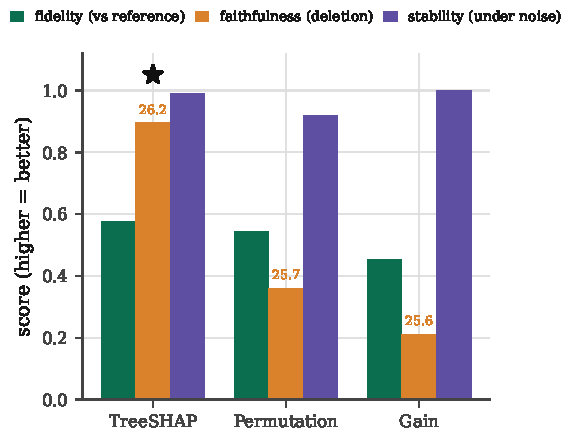
\includegraphics[width=0.99\columnwidth]{fig_audit.pdf}
\caption{Per-method explanation quality on three lenses, each scaled so that taller is better. The deletion bars are annotated with their raw area values. TreeSHAP (starred) leads on fidelity and faithfulness while remaining near-perfectly stable.}
\label{fig:audit}
\end{figure}

\begin{figure}[t]
\centering
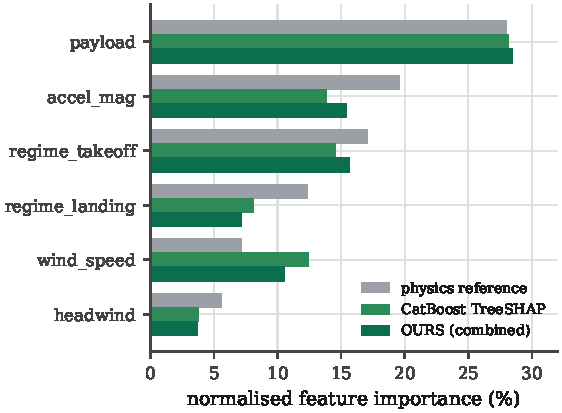
\includegraphics[width=0.99\columnwidth]{fig_importance.pdf}
\caption{Top feature importances under the physics reference, the CatBoost TreeSHAP attribution, and the ensemble's combined attribution. The three agree on payload as the dominant driver, lending the explanation operational credibility.}
\label{fig:importance}
\end{figure}

\subsection{Reconciling the Three Axes}
Whether the three rankings agree is what ultimately decides how a model should be picked, and the evidence says they do not. The Spearman correlation between the accuracy and fidelity orderings is a mere 0.14; between accuracy and robustness it is essentially nil ($-0.04$), a gap that XGBoost (accurate yet fragile) and Ridge (robust yet inaccurate) between them make vivid; and even fidelity and robustness, related at a moderate 0.54, are nowhere near interchangeable. Because no one criterion stands in reliably for the others, this is exactly the situation where multi-criteria selection pays for itself.

Read as a Pareto problem, the scorecard of Table~\ref{tab:scorecard} tells the same story, since only two models are non-dominated: Ridge, pinned at maximal fidelity and robustness, and the proposed ensemble, which combines the best accuracy, the strongest robustness among the accurate models, and a tied-best black-box fidelity. Every booster baseline, CatBoost among them, is dominated by the ensemble. Fig.~\ref{fig:uts} and Table~\ref{tab:uts} then turn this geometry, through the Unified Trust Score, into advice that depends on the mission, since the ensemble takes the performance-critical and balanced profiles outright while Ridge prevails only under the safety-critical profile, where its near-perfect fidelity and tiny noise degradation outweigh its much larger error once certification is what counts. We find this more honest than a single leaderboard, because the ensemble is the right default for nearly every mission and the lone exception, a certification-bound safety profile, is made explicit rather than blended away into one misleading number.

\begin{table}[t]
\centering
\caption{Unified Trust Score by mission profile (recommended model in bold) and Pareto membership. Cross-criterion Spearman: acc--fid $0.14$, acc--rob $-0.04$, fid--rob $0.54$.}
\label{tab:uts}
\small
\begin{tabular}{@{}lcccc@{}}
\toprule
Model & Perf. & Balanced & Safety & Pareto \\
\midrule
RAS (ours) & \best{0.80} & \best{0.67} & 0.55 & \checkmark \\
CatBoost & 0.76 & 0.62 & 0.50 & \\
Gradient Boosting & 0.69 & 0.56 & 0.44 & \\
LightGBM & 0.69 & 0.53 & 0.42 & \\
Random Forest & 0.62 & 0.48 & 0.35 & \\
XGBoost & 0.61 & 0.41 & 0.32 & \\
Ridge & 0.40 & 0.66 & \best{0.80} & \checkmark \\
\bottomrule
\end{tabular}
\end{table}

\begin{figure}[t]
\centering
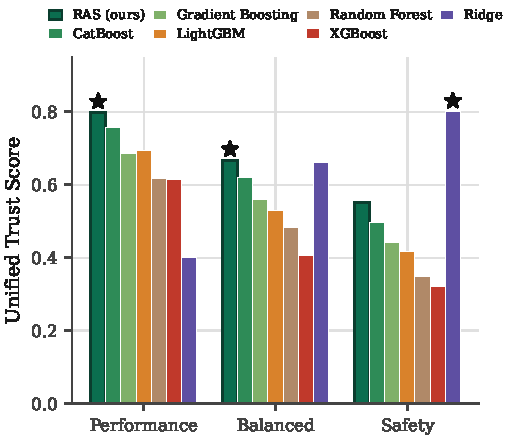
\includegraphics[width=0.99\columnwidth]{fig_uts.pdf}
\caption{Unified Trust Score across three mission profiles. A star marks the recommended model per profile: the proposed ensemble for performance-critical and balanced missions, Ridge once certification-grade fidelity and robustness dominate.}
\label{fig:uts}
\end{figure}

\section{Discussion}

\subsection{From Audit to Deployment}
An audit only helps if it reaches the operator, and Fig.~\ref{fig:deploy} sketches a serving architecture that carries all three axes into production: a client posts flight context to a REST service, an ensemble stage returns the power estimate, a consensus stage attaches the audited attribution, and an assistant stage renders it as a short natural-language rationale~\cite{molnar2022interpretable}. Crucially, the faithfulness audit runs offline and picks the explainer served at run time, so the operator sees the explanation the audit already vetted rather than an arbitrary one, and what comes back is a triple of prediction, attribution, and rationale rather than a lone number.

\begin{figure*}[t]
\centering
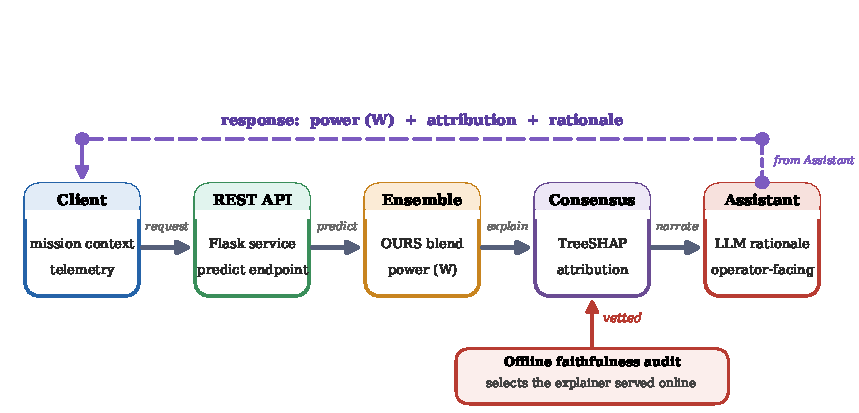
\includegraphics[width=0.95\textwidth]{fig_deploy.pdf}
\caption{Reference serving architecture. Because the offline faithfulness audit chooses the explainer used online, the deployed explanation is the vetted one, and the operator receives prediction, attribution, and rationale in a single response.}
\label{fig:deploy}
\end{figure*}

\subsection{An Operator-Facing Decision Tool}
As a front end to the same multi-criteria layer, Fig.~\ref{fig:tool} exposes it as a decision aid, where an operator sets the mission profile by weighting accuracy, fidelity, and robustness and can switch on hard constraints such as a certification requirement. In return the tool reports the recommended model, its three-axis scorecard, the rationale, and the complete ranking, and for the performance-critical profile shown it points to the proposed ensemble and explains why, namely that this model is the most accurate, that it Pareto-dominates every baseline, and that its consensus explanation names payload as the dominant driver. We keep the recommendation readable on purpose, since a tool that merely emitted the lowest-error model would walk straight back into the failure mode this paper sets out to fix.

\begin{figure*}[t]
\centering
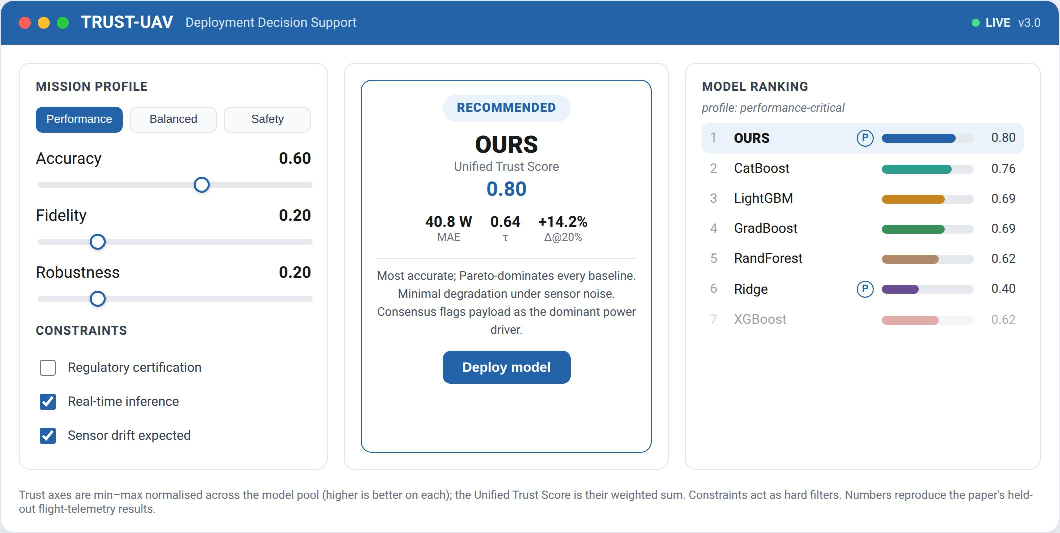
\includegraphics[width=0.80\textwidth]{fig_tool.pdf}
\caption{Operator-facing decision tool. Mission weights and constraints on the left, the recommended model with its three-axis scorecard and rationale in the centre, and the trust-ranked model list on the right.}
\label{fig:tool}
\end{figure*}

\subsection{A Digital-Twin Reading}
The framework also fits a digital-twin view of the airframe, where a faithful, robust surrogate of power draw runs continuously beside the physical vehicle. Here fidelity and robustness become operating requirements rather than niceties, since a twin whose explanations wander from physics, or whose predictions lurch with sensor noise, cannot underwrite the abort and re-route decisions it exists to inform, and our Pareto set gives such a twin a defensible menu to choose from.

\subsection{Limitations}
Several caveats naturally temper these conclusions, beginning with the fidelity reference, which is a linear surrogate: the near-linear dominance of payload justifies it well here, yet it will understate any truly non-linear interaction, and that is part of why we pair it with the reference-free deletion criterion rather than leaning on it alone. The ensemble's accuracy advantage, consistent though it is across splits, remains small, and the Wilcoxon floor at five seeds blocks a sharper significance claim that a larger seed budget would sharpen. Our robustness probe, moreover, relies on isotropic Gaussian noise, which stands in for real sensor degradation without pretending to model it~\cite{hendrycks2019benchmarking}. Because the results also come from a single airframe and data set, the procedure should carry over even where the exact rankings do not.

\section{Future Work}
Beyond these limits, the framework invites several extensions, the most immediate of which again concerns the fidelity reference, since as a single linear surrogate it could give way to a richer one, such as a physics-informed energy model~\cite{abeywickrama2018comprehensive} or an ensemble of surrogates, tested against a less restrictive ground truth. Because the trust axes are moreover point estimates, pairing the predictor with conformal prediction~\cite{vovk2005algorithmic} would hang distribution-free uncertainty on each power estimate and let the abort decision reason about predictive risk directly. Our probe, in turn, perturbs inputs at random, whereas explanations themselves can be attacked~\cite{slack2020fooling}, so testing the served attribution under adversarial rather than merely random perturbation is a natural way to harden it. Instance-level diagnostics such as influence functions~\cite{koh2017understanding} would go further and localise which training flights most shape a given prediction, complementing the global attributions used here. Finally, because the rankings rest on one airframe and data set, repeating the three-axis audit across airframes and flight envelopes would separate the conclusions that are universal from those specific to the platform.

\section{Conclusion}
Our argument has been that choosing a UAV power model on accuracy alone is unsafe for a safety-relevant deployment, and we have put a concrete alternative in its place: audit accuracy, explanation fidelity, and robustness together, then decide with a transparent multi-criteria rule. On real flight telemetry, Robust Anchored Stacking Pareto-dominates every black-box baseline, being the most accurate model on every split, the most robust of the accurate models, and tied for the most faithful black box, while the explainer choice proved to matter, with TreeSHAP the clear pick and an accurate but brittle booster caught buckling under noise the accuracy column had hidden. Because the three axes disagree, the model to deploy still depends on the mission, and our Pareto analysis and Unified Trust Score make that dependence explicit and usable rather than averaging it out of sight, so the message we hope outlives the particular numbers is simple: trustworthy deployment is a multi-criteria decision, and the lowest error is only one term in it.

\appendix
\subsection{Unified Trust Score}
We first min--max normalise the three axis scores across the model pool so that higher is better on each: accuracy becomes $1-\widetilde{\mathrm{MAE}}$, fidelity becomes $\tilde\tau$, and robustness becomes $1-\widetilde{\Delta}$, all in $[0,1]$, with a tilde marking the pool-wise normalised value. Given a mission profile with weights $(w_a,w_f,w_r)$ that sum to one, the Unified Trust Score is the weighted sum $\mathrm{UTS}=w_a s_a + w_f s_f + w_r s_r$. The three profiles take $(0.60,0.20,0.20)$ for performance-critical, $(0.34,0.33,0.33)$ for balanced, and $(0.20,0.50,0.30)$ for safety-critical missions, and the recommendation is whichever model maximises UTS subject to any active hard constraint.

\subsection{Reproducibility}
Every experiment uses the public DJI Matrice 100 data set~\cite{rodrigues2021drone}, partitioned by flight identifier into an $80/20$ grouped split so that no flight sits in both train and test. Multi-seed accuracy is averaged over five leakage-free splits and the robustness curves over ten noise draws per level, and all models use scikit-learn~\cite{pedregosa2011scikit} with the matching gradient-boosting libraries. For double-blind review, the complete code, configurations, and regeneration scripts are provided in an anonymised repository at \url{https://anonymous.4open.science/r/RAS-UAV-audit/}, where fixed seeds reproduce every reported number exactly and pinned open-source dependencies keep the CPU-only pipeline portable across machines.

\bibliographystyle{IEEEtran}
\bibliography{refs}

\end{document}
